\documentclass[14pt,a4paper]{scrartcl}
%\usepackage[14pt]{extsizes}
\usepackage[utf8]{inputenc}
\usepackage[english,russian,ukrainian]{babel}
\usepackage{indentfirst}
\usepackage{misccorr}
\usepackage{graphicx}
\usepackage{amsmath}
\usepackage{ upgreek }
\usepackage{ verbatim }

\graphicspath{}
\DeclareGraphicsExtensions{.jpg}

\begin{document}
	\begin{titlepage}
		\begin{center}
			\small{Міністерство освіти та науки України}\\
			\small{Київський національний університет імені Тараса Шевченка}\\
		\end{center}
			\vspace{15em}
		\begin{center}
			\large{Звіт}\\
			\large{До лабораторної роботи №1}\\
			\large{«Розв’язок граничної задачі для звичайного}\\
			\large{диференціального рівняння  другого порядку методом}\\
			\large{Скінченних елементів на базі методу Бубнова-Гальоркіна}\\
			\large{та інтегро-інтерполяційним методом»}\\			
		\end{center}
			
		\vspace{10em}
		

	
		\begin{flushright}
			Студента 4 курсу\\
			Факультету кібернетики\\
			Групи ОМ-4\\
			Кравця Олексія\\
			
		\end{flushright}
		
		\vspace{\fill}

		
		\begin{center}
			\small{Київ, 2019}
		\end{center}
	
	\end{titlepage}


	\newpage

	\section{Постановка Задачі}
	Методом Скінченних елементів і Інтегро-інтерполяційним методом розв'язати граничну задачу для звичайного диференціального рівняння другого порядку, та порівняти результат з вже отриманим результатом роботи методу Бубнова-Гальоркіна.

	
	\begin{equation}\label{eq1}
		\begin{cases}
			-\frac{d}{dx}(p(x)\frac{du}{dx})+a(x)\frac{du}{dx}+q(x)u=f(x)  \\ 
			h_1y(0) - h_2y'(0) =0 \\
			H_1y(1) - H_2y'(1) =0 \\
			0<x<1\\
		\end{cases}
	\end{equation}
	
	\begin{gather}
	p(x)= 2-sin(\pi x)\\
	a(x)= sin(\pi x)\\
	q(x)= 5\\
	f(x) = 2x^2 + sin(2x)\\
	h_1 = 0, h_2 = 1\\
	H_1= 1, H_2 = 4
	\end{gather}
	Розв'язати задачу при $N=50, 100$ двома методами та порівняти результати з попередньою лабораторною роботою.
	
	\section{Теоретичні відомості}
	\subsection{Метод Скінченних різниць}
	Розглянемо систему \ref{eq1}, помножимо диференціальне рівняння на $v(x)$ та проінтегруємо.
	
	\begin{equation} \label{eq2}
	\int_{0}^{1} \left[ -(p u')' + au' + qu\right]v dx = \int_{0}^{1} fv dx
	\end{equation}
	Проінтегруємо ліву частину \ref{eq2} за частинами.
	\begin{equation} \label{eq3}
	\int_{0}^{1} \left[ pu'v' + au'v + quv\right] dx - pu'v\big|_{0}^{1} = \int_{0}^{1} fv dx
	\end{equation}
	
	\begin{equation} \label{eq4}
	\int_{0}^{1} \left[ pu'v' + au'v + quv\right] dx - pu'v\big|_{0}^{1} = \int_{0}^{1} fv dx
	\end{equation}
	Нехай $h_2 \neq0, H_2 \neq0$
	\begin{equation} \label{eq5}
	\int_{0}^{1} \left[ pu'v' + au'v + quv\right] dx + p(1)u(1)v(1)\frac{H_1}{H_2} +p(0)u(0)v(0)\frac{h_1}{h_2} = \int_{0}^{1} fv dx
	\end{equation}
	
	Виберемо $\phi_i$ -базисні функції. Побудуємо їх.
	
	Розділимо відрізок $[0,1]$ на $N$ частин. Отримаємо послідовність $\left\{ x_{i}\right\}_{i=0}^{N}$. Де
	
	\begin{gather} \label{eq3}
	x_{i} = ih, i= \overline{0,N} \\
	h = \frac{1}{N}
	\end{gather}
	Тепер побудуємо функції $\phi_i$
	
	\begin{gather} \label{eq4}
	\phi_{i} = \left\{
	\begin{array}
	[c]{ll}%
	\frac{x-x_{i-1}}{h}, x \in [x_{i-1}, x] \\
	\frac{x_{i+1}-x}{h}, x \in [x_{i}, x_{i+1}]\\			
	0, x \notin [x_{i-1}, x_{i+1}] 
	\end{array} \right.
	\\
	\phi_{0} = \left\{
	\begin{array}
	[c]{ll}%
	0, x \geq x_1 \\
	\frac{x_{i}-x}{h}, 0 \leq x < x_1
	\end{array}  \right.
	\end{gather}
	
	 Розв'язок  задачі \ref{eq1} буде мати вигляд:
	
	\begin{equation} \label{eq2}
	u \approx u_N = \sum_{i=0}^{N}c_{i}\phi_{i}
	\end{equation}
	
	
	Запишемо задачу у операторному вигляді. 
	\begin{equation} \label{eq6}
	\left(Lu,v\right) = \left(f,v\right)
	\end{equation}
	
	\begin{equation} \label{eq7}
	u \approx u_N = \sum_{i=1}^{N}(c_{i}\phi_{i})
	\end{equation}
	Отже
	\begin{equation} \label{eq8}
	\left(L \sum_{i=1}^{N}(c_i \phi_i), \phi_j\right) = \left(f,\phi_j\right), \forall j= \overline{1,N}
	\end{equation}
	
	\begin{equation} \label{eq9}
	\sum_{i=1}^{N}c_i\left(L\phi_i, \phi_j\right) = \left(f,\phi_j\right), \forall j= \overline{1,N}
	\end{equation}
	
	Отримали систему лінійних алгебраїчних рівнянь $Ac=F$, де $A = [a_{ji}]= \left[\left(L\phi_i,\phi_j\right)\right], F_{j}=\left(f,\phi_j\right), i,j=\overline{1,N}$
	Треба задовольнити головним умовам, в нашому випадку це умови першого типу. Відповідно покладемо $c_0 ,c_N =0$, якщо це необхідно.
	
	Помітимо
	
	\begin{equation} \label{eq5}
	\int_{0}^{1} p(x)\phi_{i}'(x)\phi_{j}'(x) \ne 0 
	\end{equation}
	
	лише коли $ \left\{
	\begin{array}{ll}
	i = j+1 \\
	i = j
	\end{array}\right.
	$
	
	Тому можемо рахувати інтеграли такого вигляду.
	
	\begin{equation} \label{eq6}
	\int_{x_{i-1}}^{x_{i+1}} p(x)\phi_{i}'(x)\phi_{i \pm 1}'(x)
	\end{equation}
	
	Також можна помітити, що отримана в результаті матриця буде тридіагональною. 
	
	\subsection{Інтегро-інтерполяційний метод}
	
	Розподілимо $[0,1]$ на $N$ частин з рівномірним кроком $h= \frac{1}{N}$, де $x_{0} = 0$, $x_{N} = 1$.
	
	Для використання методу перетворимо систему \ref{eq1} у таку форму:
	
	\begin{equation}\label{eq10}
	\left\{
	\begin{array}{ll}
		-(ku')' +qu = f,\qquad 0<x<1 \\
		-ku' + \alpha_{1}u = \mu_{1},\qquad x =0\\
		ku' + \alpha_{2}u = \mu_{2},\qquad x =1
	\end{array}\right.
	\end{equation}
	
	Для цього скористаємося формулами:
	
	\begin{equation}\label{eq11}
		k(x) = p(x)\frac{1}{e^{\int \frac{a(x)}{p(x)} dx}}
	\end{equation}

	\begin{equation}\label{eq12}
		q(x) = q(x) \frac{1}{e^{\int \frac{a(x)}{p(x)} dx}}
	\end{equation}	
	
	\begin{equation}\label{eq13}
		f(x) = f(x)\frac{1}{e^{\int \frac{a(x)}{p(x)} dx}}
	\end{equation}	
	
	\begin{equation}\label{eq14}
		\alpha_{1} = p(0)\frac{h1}{h2},\qquad h2 \ne 0
	\end{equation}
	
	\begin{equation}\label{eq15}
		\alpha_{2} = p(1)\frac{H1}{H2},\qquad h2 \ne 0
	\end{equation}


	Виходячи з інтегрального рівняння збереження тепла, запишемо:
	
	\begin{equation}\label{eq16}
		w_{i-\frac{1}{2}} + \int_{x_{i- \frac{1}{2}}}^{x_{i+\frac{1}{2}}} f(x)dx = \int_{x_{i- \frac{1}{2}}}^{x_{i+\frac{1}{2}}} q^{2}(x)u(x)dx = w_{i+\frac{1}{2}}
	\end{equation}

	\begin{equation}\label{eq17}
		-w_{i+\frac{1}{2}} + w_{i-\frac{1}{2}} - \int_{x_{i- \frac{1}{2}}}^{x_{i+\frac{1}{2}}} q^{2}(x)u(x)dx = -\int_{x_{i- \frac{1}{2}}}^{x_{i+\frac{1}{2}}} f(x)dx
	\end{equation}
	
	Де $w$ - потік тепла. Препишемо (\ref{eq17}) для зручності.
	
	\begin{equation}\label{eq18}
		w_{i+\frac{1}{2}} - w_{i-\frac{1}{2}} + \int_{x_{i- \frac{1}{2}}}^{x_{i+\frac{1}{2}}} q^{2}(x)u(x)dx = \int_{x_{i- \frac{1}{2}}}^{x_{i+\frac{1}{2}}} f(x)dx
	\end{equation}
	
		
	\begin{gather}
		w(x) = ku' \label{eq19}\\
		u' =  - \frac{w(x)}{k(x)} \label{eq20}
	\end{gather}
	
	Проінтегруємо (\ref{eq20}) по проміжку $x_{i-1}, x_{i}$:
	
	\begin{equation} \label{eq21}
		u_{i} - u_{i-1} = - \int_{x_{i-1}}^{x_{i}} \frac{w(x)}{k(x)}dx = -w(\xi)\int_{x_{i-1}}^{x_{i}} \frac{1}{k(x)}dx \approx -w_{x_{i-\frac{1}{2}}}\int_{x_{i-1}}^{x_{i}} \frac{1}{k(x)}dx	
	\end{equation}
	
	\begin{equation}\label{eq22}
		w_{x_{i-\frac{1}{2}}} \approx a_{i}u_{\overline{x}}
	\end{equation}

	\begin{equation}\label{eq23}
		a_{i} = \left( \frac{1}{h}\int_{x_{i-1}}^{x_{i}}\frac{1}{k(x)}dx \right)^{-1}
	\end{equation}

	\begin{equation}\label{eq24}
		\int_{x_{i-\frac{1}{2}}}^{x_{i+\frac{1}{2}}} q^{2}(x)u(x)dx \approx u_{i} h d_{i}
	\end{equation}
	
	
	\begin{equation}\label{eq25}
		d_{i} = \frac{1}{h}\int_{x_{i-\frac{1}{2}}}^{x_{i+\frac{1}{2}}} q(x)dx
	\end{equation}
	
	\begin{equation}\label{eq26}
		\int_{x_{i-\frac{1}{2}}}^{x_{i+\frac{1}{2}}} f(x)dx = h \phi_{i}
	\end{equation}
	
	\begin{equation}\label{eq27}
		\phi_{i} = \frac{1}{h} \int_{x_{i-\frac{1}{2}}}^{x_{i+\frac{1}{2}}} f(x)dx
	\end{equation}	
	
	Підставивши ці вирази в (\ref{eq18}) і поділивши весь вираз на $h$ отримаємо різницеву схему.
	
	
	\begin{equation}\label{eq28}
		-(a y_{\overline{x}})_{x,i} + d_{i}y_{i}  = \phi_{i}, \qquad x \in w_h 
	\end{equation}	
	
	Де $w_h$ - внутрішні вузли сітки, коеф. різницевої схеми визначаються формулами (\ref{eq23}, \ref{eq25}, \ref{eq27})	
	
	Розглянемо випадок, з крайовими умовами 3 роду.
	
	\begin{gather}
	-ku' + \alpha_{1} = \mu_{1}, \qquad x =0 \label{eq29}\\
	ku' + \alpha_{2} = \mu_{2}, \qquad x =1 \label{eq30}
	\end{gather}
	
	Розглянемо (\ref{eq29}), розглядаємо проміжок $[x_{0}, x_{\frac{1}{2}}]$:
		
	\begin{equation}\label{eq31}
		w_{\frac{1}{2}} - w_{0} + \int_{x_{0}}^{x_{\frac{1}{2}}}qudx =  \int_{x_{i}}^{x_{\frac{1}{2}}}fdx
	\end{equation}	
	
	З формули (\ref{eq22}) маємо
	
	\begin{equation}\label{eq32}
		w_{\frac{1}{2}} \approx -a_{1}u_{\overline{x},1}
	\end{equation}
	
	З (\ref{eq29}):
	
	\begin{equation}\label{eq33}
		W_{0} = \mu_{1} - \alpha_{1}u_{0}
	\end{equation}
	
	
	\begin{equation}\label{eq34}
		\int_{x_0}^{x_{\frac{1}{2}}}q(x)u(x)dx \approx u_{i}\frac{h}{2}d_{0}
	\end{equation}
	
	\begin{equation}\label{eq35}
		d_{0} \approx \frac{2}{h}\int_{x_0}^{x_{\frac{1}{2}}}q(x)dx
	\end{equation}	
	
	\begin{equation}\label{eq36}
	\int_{x_0}^{x_{\frac{1}{2}}}f(x)dx \approx \frac{h}{2}\phi_{0}
	\end{equation}
	
	\begin{equation}\label{eq37}
	\phi_{0} \approx \frac{2}{h}\int_{x_0}^{x_{\frac{1}{2}}}f(x)dx
	\end{equation}	
	
	
	Підставляючи вирази (\ref{eq32}, \ref{eq33}, \ref{eq34},\ref{eq36}) в (\ref{eq31}) отримаємо
	
	

	\begin{equation}\label{eq38}
		-a_{1}y_{x,0} + \alpha_{1}y_{0} +\mu_{1} + \frac{h}{2}d_{0}y_{0} = \frac{h}{2}\phi_{0}
	\end{equation}
	
	\begin{equation}\label{eq39}
		-a_{0}y_{x,0} + \overline{\alpha_{1}}y_{0} = \overline{\mu_{1}}
	\end{equation}
	
	Отримали фароксимацію (\ref{eq39}) де коеф. визначаються
	
	\begin{gather}
		\overline{\alpha_{1}} = \alpha_{1} +\frac{h}{2}d_{0} \label{eq40}\\
		\overline{\mu_{1}} = \mu_{1} + \frac{h}{2}\phi_{0} \label{eq41}
	\end{gather}

	Різницева апроксимація для граничних умов (\ref{eq30}) рахується аналогічно:
	
	\begin{gather}
		a_{N}y_{\overline{x},N} + \overline{\alpha_{2}}y_{N} = \overline{\mu_{2}}\label{eq42}\\
		\overline{\alpha_{2}} = \alpha_{2} +\frac{h}{2}d_{N}\label{eq43}\\
		\overline{\mu_{2}} = \mu_{2} + \frac{h}{2}\phi_{N} \label{eq44}
	\end{gather}
	
	Отримаємо систему лінійних алгебраїчних рівнянь, з тридіагональноюю матрицею. Після розв'язання системи отримаємо значення розвязку системи (\ref{eq1}) в точках $x_{i}, i = \overline{0,N}$.
	
	
	\section{Практична частина}
	
	\subsection{Метод Скінченних різниць}

	Побудуємо функції для $N = 50, N = 100$ та порівняємо з результатом метода Гальоркіна при $N = 10$:
	
	\begin{figure}[h]
		\begin{center}
			\begin{minipage}[h]{0.45\linewidth}
				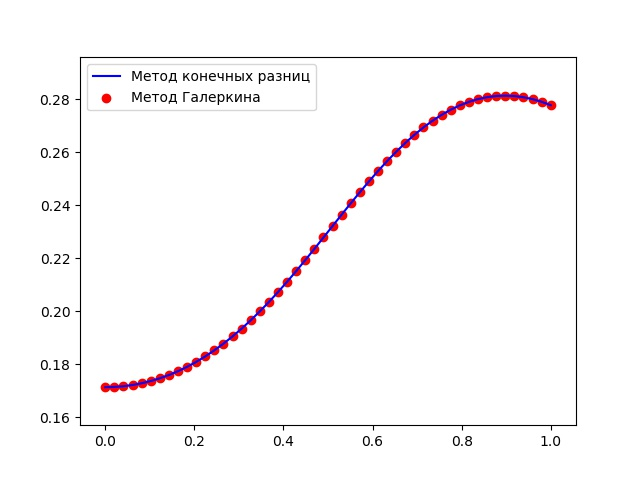
\includegraphics[width=1\linewidth]{photo1.jpg}
				\caption{$N = 50$} %% подпись к рисунку
				\label{ris:experimoriginal} %% метка рисунка для ссылки на него
			\end{minipage}
			\hfill
			\begin{minipage}[h]{0.45\linewidth}
				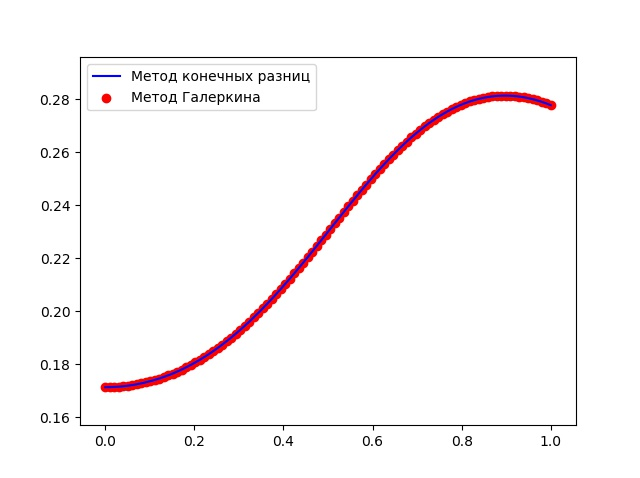
\includegraphics[width=1\linewidth]{photo2.jpg}
				\caption{$N = 100$}
				\label{ris:experimcoded}
			\end{minipage}
		\end{center}
	\end{figure}
	
	Порівняємо графіки результатів метода Скінченних різниць при $N= 50, N = 100$.
	
	\begin{figure}[h!]
		\center{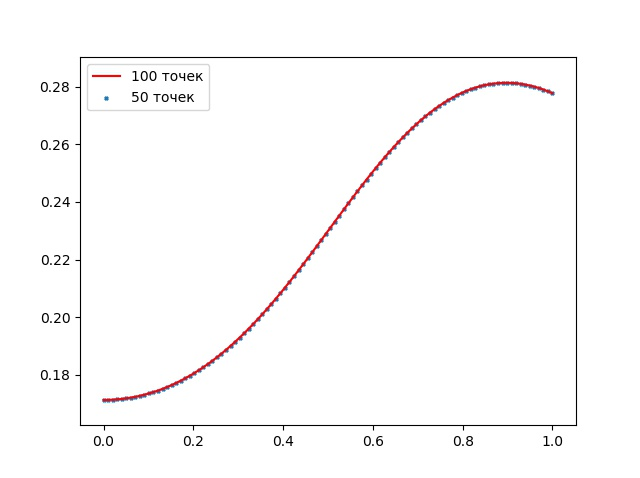
\includegraphics[scale=0.9]{photo3.jpg}}
		\caption{$N=50,N=100$}
		\label{fig:image}
	\end{figure}



	Подивимося на різницю між результатами при $N=50, N=100$:
	
	\begin{center}
		\begin{tabular}{ | c | c | }
			\hline
			$x$ & $|u_{50}(x)-u_{100}(x)|$\\ \hline
			0.00 & 0.000002 \\
			0.10 & 0.000000 \\
			0.20 & 0.000002 \\
			0.30 & 0.000003 \\
			0.40 & 0.000004 \\
			0.50 & 0.000002 \\
			0.60 & 0.000001 \\
			0.70 & 0.000003 \\
			0.80 & 0.000002 \\
			0.90 & 0.000000 \\
			1.00 & 0.000002 \\
			\hline
		\end{tabular}
	\end{center}


\subsection{Інтегро-інтерполяційний метод}
	Побудуємо функції для $N = 50, N = 100$ та порівняємо з результатом метода Гальоркіна при $N = 10$:
	
	
	\begin{figure}[h]
		\begin{center}
			\begin{minipage}[h]{0.45\linewidth}
				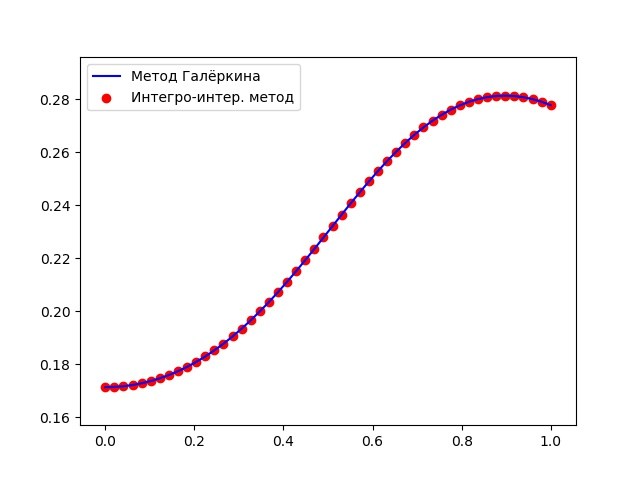
\includegraphics[width=1\linewidth]{photo1_1.jpg}
				\caption{$N = 50$} %% подпись к рисунку
				\label{ris:experimoriginal} %% метка рисунка для ссылки на него
			\end{minipage}
			\hfill
			\begin{minipage}[h]{0.45\linewidth}
				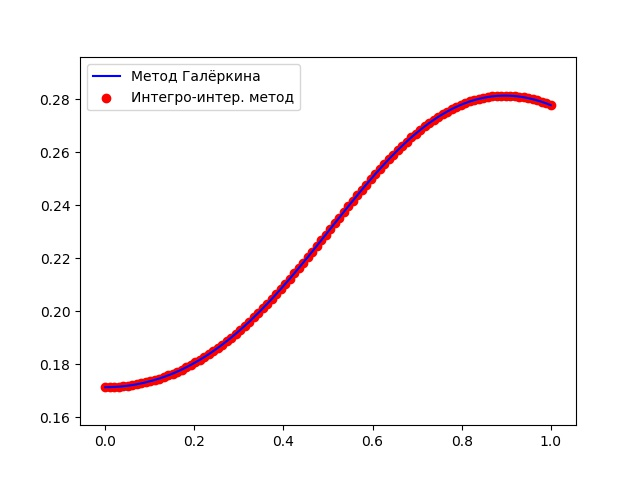
\includegraphics[width=1\linewidth]{photo2_1.jpg}
				\caption{$N = 100$}
				\label{ris:experimcoded}
			\end{minipage}
		\end{center}
	\end{figure}


	Порівняємо графіки результатів метода Скінченних різниць при $N= 50, N = 100$.
	
	\begin{figure}[h!]
		\center{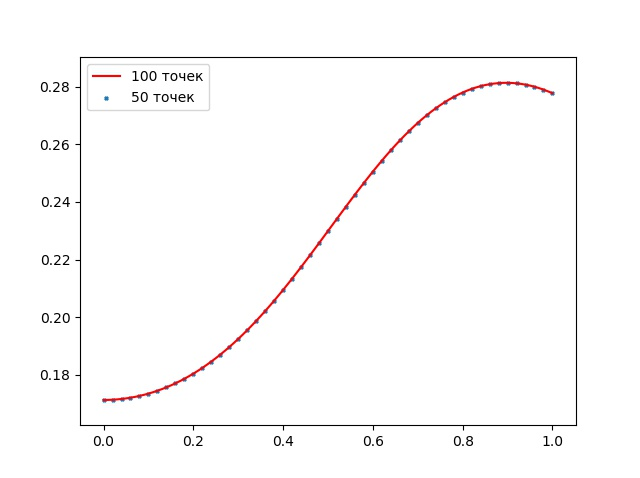
\includegraphics[scale=0.9]{photo3_1.jpg}}
		\caption{$N=50,N=100$}
		\label{fig:image}
	\end{figure}



	Подивимося на різницю між результатами при $N=50, N=100$:
	
	\begin{center}
		\begin{tabular}{ | c | c | }
			\hline
			$x$ & $|u_{50}(x)-u_{100}(x)|$\\ \hline
			0.00 & 0.000001 \\
			0.10 & 0.000001 \\
			0.20 & 0.000002 \\
			0.30 & 0.000002 \\
			0.40 & 0.000001 \\
			0.50 & 0.000000 \\
			0.60 & 0.000002 \\
			0.70 & 0.000002 \\
			0.80 & 0.000003 \\
			0.90 & 0.000002 \\
			1.00 & 0.000002 \\
			\hline
		\end{tabular}
	\end{center}
		
		
\subsection{Порівняння 3 методів}

	Розглянемо різницю результатів методу Гальоркіна при $N=10$, Методу скінченних різниць $N=100$, Ітегро-інтерполяційним метод при $N=100$
	
	
		\begin{center}
		\begin{tabular}{ | c | c | c | c | c | c | c |  }
			\hline
			$x$ & $u_0$ & $u_1$ & $u_2$ & $\delta_{0,1}$ & $\delta_{0,2}$ & $\delta_{1,2}$\\ \hline
			0.00 & 0.171333 & 0.171336 & 0.171335 & 0.000003 & 0.000002 & 0.000001\\
			0.10 & 0.173543 & 0.173545 & 0.173542 & 0.000001 & 0.000001 & 0.000003\\
			0.20 & 0.180465 & 0.180468 & 0.180464 & 0.000004 & 0.000000 & 0.000004\\
			0.30 & 0.192504 & 0.192508 & 0.192503 & 0.000004 & 0.000001 & 0.000005\\
			0.40 & 0.209514 & 0.209518 & 0.209514 & 0.000003 & 0.000000 & 0.000003\\
			0.50 & 0.229962 & 0.229961 & 0.229962 & 0.000001 & 0.000000 & 0.000001\\
			0.60 & 0.250552 & 0.250548 & 0.250553 & 0.000004 & 0.000001 & 0.000005\\
			0.70 & 0.267425 & 0.267419 & 0.267426 & 0.000006 & 0.000001 & 0.000007\\
			0.80 & 0.277967 & 0.277962 & 0.277967 & 0.000005 & 0.000001 & 0.000006\\
			0.90 & 0.281329 & 0.281326 & 0.281330 & 0.000003 & 0.000001 & 0.000004\\
			1.00 & 0.277719 & 0.277717 & 0.277719 & 0.000002 & 0.000001 & 0.000001\\
			\hline
		\end{tabular}
	\end{center}
	
	Де $u_0$- результат методу Гальоркіна, $u_1$-результат методу Скінченних різниць, $u_2$ - результат Інтегро-інтерполяційного методу,  $\delta_{0,1}$ різниця між $u_{0}, u_{1}$,  $\delta_{0,2}$ різниця між $u_{0}, u_{2}$,  $\delta_{1,2}$ різниця між $u_{1}, u_{2}$
\end{document}